    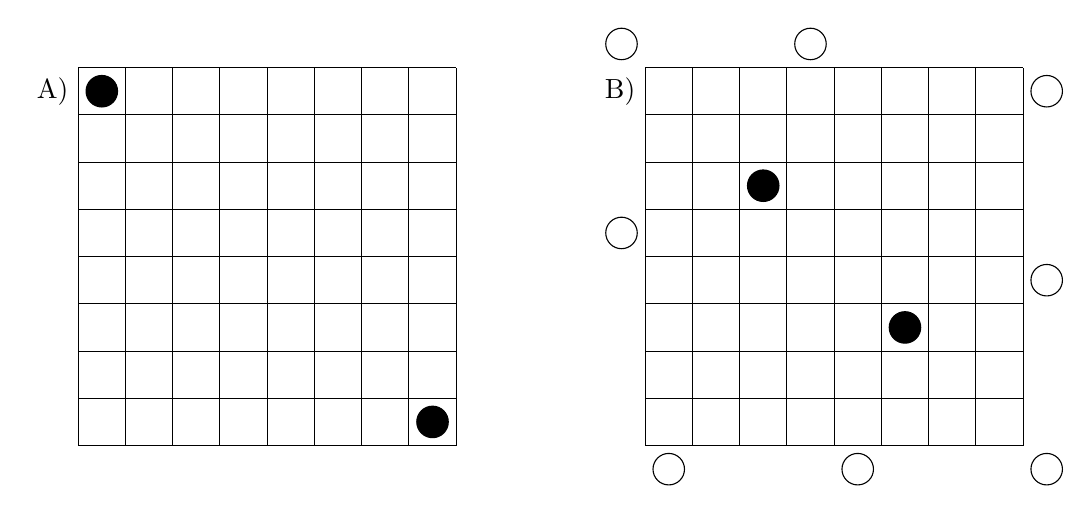
\begin{tikzpicture}
        \node[anchor = north east] (A) at (0.0,4.8) {A)};
        \node[anchor = north east] (B) at (7.2,4.8) {B)};
        
        \draw[scale = 0.6, thin] ( 0,0) grid (8,8);
        \draw[scale = 0.6, thin] (12,0) grid (20,8);
        %\coordinate[label = A] (a) at (0.3,0.05);

        % board 1 (2 replicates)
        \filldraw[black] (0.3,4.5) circle (0.2);
        \filldraw[black] (4.5,0.3) circle (0.2);

        % board 2 (2 replicates + 8 fake edge wells)
        \filldraw[black] (10.5, 1.5) circle (0.2);
        \filldraw[black] ( 8.7, 3.3) circle (0.2);
        \draw            ( 6.9, 5.1) circle (0.2); %0,                            0,
        \draw            ( 7.5,-0.3) circle (0.2); %num_rows_line + 1,            1,
        \draw            (12.3, 4.5) circle (0.2); %1,                            num_cols_line + 1,
        \draw            (12.3,-0.3) circle (0.2); %num_rows_line + 1,            num_cols_line + 1
        \draw            ( 9.3, 5.1) circle (0.2); %0,                            floor(num_cols_line / 2),
        \draw            (12.3, 2.1) circle (0.2); %floor(num_rows_line / 2) + 1, num_cols_line + 1,
        \draw            ( 9.9,-0.3) circle (0.2); %num_rows_line + 1,            floor(num_cols_line / 2) + 1,
        \draw            ( 6.9, 2.7) circle (0.2); %floor(num_rows_line / 2),     0 
    \end{tikzpicture}
